\documentclass[11pt]{article}
\usepackage[a4paper,margin=22mm]{geometry}
\usepackage[T1]{fontenc}
\usepackage{lmodern}
\usepackage{microtype}
\usepackage{graphicx}
\usepackage{booktabs}
\usepackage{array}
\usepackage{enumitem}
\usepackage[numbers,sort&compress]{natbib}
\usepackage[dvipsnames]{xcolor}
\usepackage{hyperref}
\usepackage{xurl}
\usepackage{flafter}
\usepackage[section]{placeins}
\ifdefined\pdfinfoomitdate\pdfinfoomitdate=1\fi
\ifdefined\pdftrailerid\pdftrailerid{}\fi
\ifdefined\pdfsuppressptexinfo\pdfsuppressptexinfo=15\fi
\hypersetup{colorlinks=true,linkcolor=MidnightBlue,citecolor=MidnightBlue,urlcolor=MidnightBlue,pdftitle={From Configurations to Claims: An Evidence Audit of Urban EV Charging Forecasting},pdfauthor={Hongwei Chi},pdfsubject={Audit of experimental evidence in urban EV charging forecasting},pdfkeywords={electric vehicle charging, forecasting, reproducibility, experiment audit, latency, stopping rules}}
\setlist{nosep,leftmargin=*}
\setlength{\emergencystretch}{3em}
\newcommand{\urbanev}{UrbanEV}
\newcommand{\rmse}{RMSE}
\title{From Configurations to Claims:\\An Evidence Audit of Urban EV Charging Forecasting}
\author{%
FreeSakura%
}

\newcommand{\provisionalauthorshipnote}{%
\begin{center}
\footnotesize\emph{Public attribution uses the contributor's pseudonym. Formal submission authorship will be finalized separately.}
\end{center}}

\date{Working draft after v0.9.1}
\begin{document}
\maketitle
\provisionalauthorshipnote
\begin{abstract}
A completed run does not necessarily reproduce the experiment described in a paper. Likewise, a positive comparison does not always justify another round of model development. We examine both issues in an audit of urban electric-vehicle charging forecasting experiments. In a frozen inventory of 1,224 UrbanEV configurations, 865 have completed artifacts, but only 156 meet the joint exact-protocol-and-numerical criterion. Under the same UrbanEV protocol, strict prequential fusion of a locally audited CAPER expert and compact TimeXer lowers internal macro RMSE by 3.178\% relative to the strongest evaluated single model. It also increases batch-1 median synchronous latency by 48.86\% on the frozen device. The learned router, Chronos-2 teacher screen, and residual-distillation experiment do not meet their predefined progression rules. On a separate Paris development-only panel, the teacher improves RMSE consistently, but its 0.847\% point gain remains below the frozen 1\% rule. Paris formal and protected target-bearing sources are stored separately and contribute no analytical result. We report these outcomes with six configuration states, locked decision rules, and artifact records. In this study, fixed fusion improves internal RMSE at a measured latency cost, and the later experiments stop under their predefined rules. The results do not establish protected-test performance, deployment readiness, or state-of-the-art performance.
\end{abstract}
\noindent\textbf{Keywords:} electric-vehicle charging; forecasting; reproducibility; prequential evaluation; experiment audit; latency; stopping rules
\section{Introduction}
\label{sec:introduction}

An experiment can finish without reproducing the claim it appears to test.  A run may emit a checkpoint and a metric even when the source protocol does not uniquely determine the target, split, preprocessing, or hyperparameters.  Conversely, a faithfully specified method may fail for an ordinary engineering reason and never yield a comparable number.  Treating these outcomes as one binary label---``reproduced'' or ``not reproduced''---hides the evidence needed to interpret a forecasting benchmark.

This distinction is consequential in urban electric-vehicle (EV) charging forecasting.  Open resources now cover zonal charging demand in Shenzhen, station occupancy in Paris, workplace charging sessions, and harmonized measurements across cities and continents \cite{li2025urbanev,amaraouali2024smarter,amaraouali2023parisdataset,lee2019acndata,guo2025charged}.  These resources do not define interchangeable prediction problems: occupancy rates, port states, session records, charging duration, and energy volume have different denominators, missingness mechanisms, and operational meanings.  At the same time, the associated modeling literature spans physics-informed graph networks, language-model formulations, exogenous-variable Transformers, linear decompositions, and pretrained forecasters \cite{qu2024pag,qu2024chatev,wang2024timexer,zeng2023dlinear,ansari2024chronos,ansari2025chronos2}.  A reported score therefore becomes interpretable only after the data semantics, information set, forecast origin, and evaluation protocol are fixed.

Forecasting research has long emphasized out-of-sample and rolling-origin evaluation \cite{dawid1984prequential,tashman2000oos}.  More recent guidance documents leakage through preprocessing, inappropriate random splits, weak benchmarks, and metric choices that do not match the data or decision problem \cite{hewamalage2023pitfalls,kapoor2023leakage}.  Reproducibility programs likewise encourage code, data, environment, and reporting artifacts \cite{pineau2021reproducibility}.  These practices are necessary, but a remaining gap is operational: once a large matrix has been partially recovered and executed, how should a researcher distinguish disclosure quality from execution status, predictive opportunity from realizable gain, and a statistically detectable difference from an improvement large enough to justify added serving cost?  Without explicit distinctions, additional model search can gradually convert an evaluation interval into a tuning resource.

We address this gap through an artifact-grounded case audit of one UrbanEV forecasting inventory and its subsequent model-development chain.  The intended readers are benchmark authors, artifact evaluators, and reviewers who must decide which urban-forecasting claims are licensed by a heterogeneous experiment record.  The audit freezes a six-state configuration taxonomy, verifies target and run identities, and follows each proposed improvement through a sequential evidence ladder.  That ladder separates an infeasible oracle diagnostic, forecast-origin predictability, strict prequential fixed fusion, learned routing, synchronous latency, foundation-model teacher qualification, residual distillation, and development-only replication on a separately isolated Paris panel.  Fail-closed metric locks prevent incomplete or invalid artifacts from entering aggregate results, while internally time-stamped minimum-effect gates determine whether a stage authorizes the next one.  The contribution is an auditable claim grammar and workflow instantiated by this case, not evidence that the framework has already reduced false discoveries across independent teams.

The audit changes the apparent story.  Of 1,224 frozen configurations, 865 have completed artifacts, but only 156 satisfy the joint exact-protocol-and-numerical criterion.  In the internal UrbanEV rolling evaluation, a strictly fitted CAPER--TimeXer fusion reduces macro RMSE by 3.178\% relative to the strongest evaluated single model, yet increases batch-1 median synchronous latency by 48.86\% on the frozen laptop-GPU workload.  A learned router adds only 0.443\% over that fixed reference and therefore fails the internally time-stamped 1\% progression gate despite a positive block-bootstrap interval.  The same discipline rejects Chronos-2 as the project teacher under the exact UrbanEV protocol, stops residual distillation after a 0.119\% gain over ground-truth-only training, and withholds student training on Paris when a strict development-only teacher improves by 0.847\% rather than the required 1\%.  These are scoped gate outcomes, not general verdicts about routing, foundation models, or distillation.

We organize the study around four research questions:

\begin{enumerate}
    \item[\textbf{RQ1}] How much of a large forecasting configuration matrix is exactly reproducible, approximately recoverable, trend-only, underidentified, failed, or never completed?
    \item[\textbf{RQ2}] When two experts are complementary, how much of an infeasible oracle gap survives strict prequential fixed fusion and learned routing?
    \item[\textbf{RQ3}] How do apparent accuracy gains change once synchronous inference latency and a frozen minimum-effect threshold are enforced?
    \item[\textbf{RQ4}] How do fail-closed audits, control branches, independent evidence, and stopping rules change the claims that remain defensible?
\end{enumerate}

This paper makes four contributions:

\begin{itemize}
    \item \textbf{A configuration-level evidence taxonomy.}  We separate protocol and numerical reproduction, disclosure-limited recovery, trend-only recovery, underidentification, execution failure, and non-completion for a frozen 1,224-configuration inventory.  The resulting registry makes clear why execution completion is not a substitute for exact reproduction.
    \item \textbf{A portable audit framework and claim grammar.}  We type evidence objects as configuration, prediction, target, metric, latency, or protected-storage artifacts; attach identity and lock requirements; and specify the narrow wording each evidence state authorizes.  A claim-to-artifact ledger and reviewer checklist make the framework inspectable rather than leaving it as project history.
    \item \textbf{A sequential audit of model-improvement claims.}  We connect target-identity checks, prequential fitting, control branches, block-resampled uncertainty, and hardware-specific latency to explicit authorization gates.  This exposes where theoretical complementarity becomes a material fixed-fusion gain and where later routing, teacher, and distillation signals remain below their frozen effect requirements.
    \item \textbf{A fail-closed evidence boundary.}  We document audit events that blocked invalid shuffled controls and repaired missing-target representation before metric access, and we procedurally isolate Paris formal and protected target-bearing sources so that only development targets contribute analytically.  The workflow produces an auditable mapping from each numerical statement to its protocol, artifact, and permitted wording.
\end{itemize}

\begin{figure}[htbp]
    \centering
    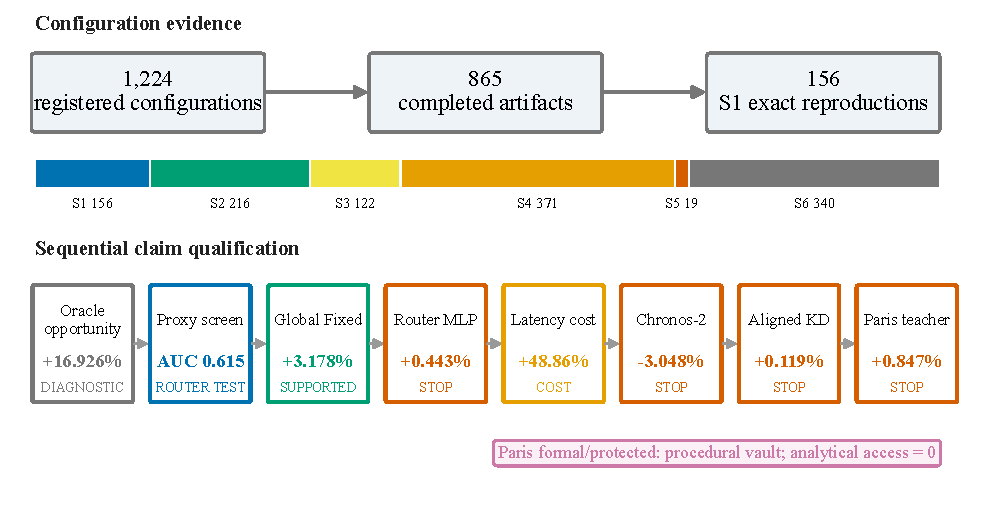
\includegraphics[width=0.9\linewidth]{figures/fig01_evidence_ladder.pdf}
    \caption{The audit separates registration, completed execution, exact reproduction, predictive opportunity, measured engineering cost, and qualification.  A positive diagnostic or comparison does not automatically authorize the next stage; Paris formal and protected targets remain in procedural vault-only storage with zero analytical use.}
    \label{fig:evidence-ladder}
\end{figure}

\paragraph{Claim boundary.}
This is an empirical audit and evaluation study, not a new state-of-the-art model paper.  Its numerical conclusions concern one UrbanEV inventory, six internal rolling folds at seed 42, one frozen latency platform, and Paris development-only evidence.  UrbanEV and Paris absolute RMSE values are not compared because the panels and targets differ.  The 1\% threshold is an internally time-stamped project convention, not a universal definition of scientific or economic significance.  Neither Paris formal nor Paris protected targets are accessed analytically, and we make no claim of protected-test performance, production readiness, universal generalization, or cross-dataset superiority.  Their movement into independent vault-only storage is recorded as a storage event rather than concealed as non-materialization.  Within that boundary, the case shows how configuration identifiability and sequential evidence controls constrain the claims this forecasting program can support.

The remainder of the paper first relates this audit to EV forecasting resources, time-series evaluation, and reproducibility research.  It then defines the evidence taxonomy and sequential protocol, reports the registry and model-chain results, analyzes the fail-closed events and claim boundaries, and concludes with implications for auditable forecasting studies.

\section{Related Work}
\label{sec:related-work}

\paragraph{EV charging data and prediction.}
Public EV charging datasets use different observation units and prediction targets.  ACN-Data records workplace charging sessions and supports behavioral and charging-control analyses \cite{lee2019acndata}.  UrbanEV provides hourly and finer-resolution zonal charging measurements for Shenzhen, together with prices, weather, points of interest, and spatial descriptors \cite{li2025urbanev}.  CHARGED combines charging duration, volume, price, weather, and geospatial fields from six cities \cite{guo2025charged}.  The Paris Smarter Mobility dataset records the states of 273 charging points at 91 stations and supports occupancy forecasting at station, area, and global levels \cite{amaraouali2024smarter,amaraouali2023parisdataset}.  These datasets support different EV forecasting tasks, but their targets are not directly comparable.  A session, an hourly charging-duration total, a zonal occupancy ratio, and a non-available-port rate require different denominators and masks.  We therefore check the target used in each experiment and compare absolute errors only within the same protocol.

The target also depends on the intended use.  Reviews of open EV load data distinguish session arrivals, connection and charging durations, energy, station load, and occupancy.  Other studies consider infrastructure siting, capacity planning, grid operation, and charging schedules \cite{amaraouali2021review,rashid2024survey}.  Forecasts may be produced at several aggregation levels or as distributions instead of point estimates.  For example, Buzna et al. use information across lower- and higher-level series for hierarchical probabilistic station-load forecasting \cite{buzna2021hierarchical}.  These differences mean that the target, aggregation level, forecast type, and horizon must be recorded as part of each protocol.  These fields define the valid comparisons in this study.  The hierarchical example is background rather than a model contribution of this paper.

Recent EV forecasting studies use several model families.  Physics-informed graph learning adds spatial structure and a price--demand prior to regional demand prediction \cite{qu2024pag}.  ChatEV treats heterogeneous charging inputs as a text-to-text prediction problem \cite{qu2024chatev}.  TimeXer combines endogenous temporal patches with exogenous variables \cite{wang2024timexer}, whereas DLinear provides a simpler decomposition and linear-projection reference for long-horizon forecasting \cite{zeng2023dlinear}.  Cross-paper ranking is outside scope because the tasks, data, splits, and metrics differ.  The compact TimeXer and CAPER models in this study are the specific local implementations recorded in our artifacts.  Our comparison keeps the target, history, horizon, fold, and evidence source the same.

\paragraph{Time-series evaluation.}
Prequential evaluation tests each forecast using only information available before its target is observed \cite{dawid1984prequential}.  Rolling-origin evaluation applies this rule at a sequence of forecast origins and may refit the model between test periods \cite{tashman2000oos}.  Cross-validation for dependent data requires care because its validity depends on the prediction setup, stationarity, and residual dependence \cite{bergmeir2012cv}.  Temporally ordered out-of-sample estimators are especially useful under realistic non-stationarity \cite{cerqueira2020evaluation}.  Our fixed-fusion and routing experiments follow the same rule: labels from the current evaluation fold are not used to fit that fold's fusion weights or router.

Metric choice also affects the meaning of a reported error.  Forecast metrics emphasize different scales, denominators, and target properties, so no single percentage error works for every task \cite{hyndman2006measures}.  Common problems include missing simple baselines, full-series preprocessing, mismatched horizons, and unsuitable aggregation \cite{hewamalage2023pitfalls}.  Forecasting competitions show the value of careful validation and model combinations, but they also show that complex systems do not always beat simple references \cite{makridakis2022m5}.  We apply the same checks when deciding whether an experiment should continue.  The target must match, the candidate must beat the locked reference, and every registered gate condition must pass.

\paragraph{Reproducibility and evidence auditing.}
Machine-learning reproducibility programs emphasize code, data, environment details, and structured checklists \cite{pineau2021reproducibility}.  Leakage can still cross a nominal train--test boundary through preprocessing, feature construction, temporal misalignment, or repeated analysis \cite{kapoor2023leakage}.  Results may also change with data sampling, initialization, and hyperparameter selection, so small score differences can be dominated by uncontrolled variation \cite{bouthillier2021variance}.  We therefore record run fingerprints, source hashes, and target-array checks.  We also label real-target metrics, proxy metrics, oracle diagnostics, latency measurements, and artifact checks separately.

Our stopping rules address changes made after results have been inspected.  A model-selection rule can be overfit even when the estimator used inside it is unbiased \cite{cawley2010selectionbias}.  Repeated use of a holdout set also weakens its role as fresh evidence \cite{dwork2015reusableholdout}.  In this project, thresholds were fixed before aggregate access, metrics stayed locked until artifacts closed, invalid controls were rerun as a full set, and later formal and protected periods remained separate.  This study documents how the stopping rules were applied and what the resulting records support; it does not introduce a new statistical test.

\paragraph{Ensembling, foundation forecasters, and distillation.}
Forecast combinations often improve accuracy because the component models make different errors.  The M5 competition provides large-scale evidence for both simple and learned combinations \cite{makridakis2022m5}.  An oracle that selects the better expert after seeing the target is still only an upper bound.  It does not show that information available at the forecast origin can recover the same gain.  We first measure this oracle bound, then test fixed fusion and learned routing without access to current-fold targets.  We also measure synchronous latency to determine the cost of running both experts.

A pretrained forecaster still needs to be tested under the target protocol.  Chronos reports zero-shot probabilistic forecasting across varied tasks \cite{ansari2024chronos}, and Chronos-2 extends this approach to grouped multivariate series and covariates \cite{ansari2025chronos2}.  However, a published aggregate ranking does not determine whether a model is a suitable teacher for a different target, context length, covariate policy, and point-forecast rule.  We therefore test one locked Chronos-2 checkpoint under the UrbanEV protocol instead of importing a reported score.

Distillation depends on teacher quality, student capacity, target alignment, and the ground-truth loss.  We compare the aligned teacher branch with an identical ground-truth-only student and a shuffled-teacher control.  Beating the shuffled control can show that the aligned teacher carries sample-specific information, but it does not establish an improvement over ground-truth training.  This comparison follows warnings about selection bias and benchmark variance \cite{cawley2010selectionbias,bouthillier2021variance}.  The experiment evaluates one fixed student under the registered gate.  Cache construction and student expansion stop when the required conditions fail.

\section{Methods}
\label{sec:methods}

\subsection{Audit design and record priority}
\label{sec:methods-audit-design}

We treated this study as an audit of existing experimental records, not as a search for a new state-of-the-art model.  Each result was linked to its protocol, configuration fingerprint, run status, prediction and target identities, metric definition, and allowed claim.  When records conflicted, final decision and summary files checked by a separately instantiated automated artifact audit took precedence over canonical result tables.  The tables took precedence over frozen protocol thresholds and historical logs.  Completed configurations were reused.  Failed or unexecuted configurations could enter later work only under a new versioned identifier, so a later run could not overwrite the earlier status.

The audit separated four questions.  \emph{Identifiability} asks whether the disclosed experiment determines a unique protocol and configuration.  \emph{Execution} asks whether that configuration reached a terminal run with an artifact.  \emph{Predictive evidence} asks whether predictions were evaluated against dataset targets under a time-respecting split.  \emph{Engineering qualification} asks whether the effect passed the minimum-effect rule and all consistency checks.  Proxy labels were used only to predict which expert would win locally.  They were not treated as forecast-accuracy evidence.

\begin{table}[t]
\centering
\caption{Compact claim-control framework. Full schemas and wording grammar are provided in the Supplementary Material.}
\label{tab:audit-framework-compact}
\footnotesize
\begin{tabular}{>{\raggedright\arraybackslash}p{0.19\linewidth}>{\raggedright\arraybackslash}p{0.36\linewidth}>{\raggedright\arraybackslash}p{0.34\linewidth}}
\toprule
Evidence object & Required control & Strongest released claim \\
\midrule
Configuration & protocol identity, disclosure mapping, execution state & registered, executed, failed, or S1--S6 evidence state \\
Prediction/target & index, time, entity, mask, and value hashes & internal/development metric for the named cell only \\
Diagnostic/proxy & target-dependent or proxy role stated explicitly & opportunity bound or predictability screen, not forecast gain \\
Engineering measure & device, precision, workload, batch, synchronization & measured latency/throughput on the frozen serving graph \\
Gate/repair & metric lock, conjunctive decision, parent/child hashes & gate pass/fail or artifact-integrity statement \\
Protected evidence & role, storage state, access definition and counter & procedural separation and zero analytical use after lock \\
\bottomrule
\end{tabular}
\end{table}


Table~\ref{tab:audit-framework-compact} summarizes the checklist used in this case.  For each claim, it records the supporting artifact, identity checks, lock or gate, and strongest allowed wording.  The checklist comes from one project and has not been validated as a general method for reducing false discoveries.  The Supplementary Material gives the full claim ledger and lock fields.

\subsection{Six-level configuration taxonomy}
\label{sec:methods-taxonomy}

We reclassified a frozen inventory of 1,224 UrbanEV configurations into six mutually exclusive evidence states.  The priority order was execution fact (S5 or S6), non-identifiability (S4), and then numerical agreement (S1--S3).

\begin{description}
    \item[S1: protocol and numerical result identifiable and reproduced.] The run covered all six folds, followed the official-compatible protocol, and each of the four disclosed metrics differed by at most 2\% from its mapped reference.
    \item[S2: protocol broadly consistent, with disclosure differences.] The run completed and remained above trend-only evidence, but used an audited correction or had a 2--5\% numerical discrepancy.
    \item[S3: relative trend only.] At least one core metric differed by more than 5\%, or the disclosed comparison cell could not be covered completely.
    \item[S4: original information insufficient for a unique configuration.] The paper omitted an identifying element, such as node identity, or an extended configuration could not be mapped uniquely to a disclosed paper cell.
    \item[S5: configuration identified but execution failed.] The manifest fixed a configuration, but the registry recorded a failed terminal state.
    \item[S6: runnable configuration not actually completed.] The manifest froze a runnable configuration that was skipped or never registered as a completed run.
\end{description}

S1--S4 can all have completed artifacts; only S1 denotes exact protocol-and-numerical reproduction under these frozen rules.  Classification was deterministic, not an inter-rater coding study.  The exact decision rules, priority order, one example per state, and reason fields are given in the Supplementary Material.  We did not change the numerical tolerances to alter the counts.  The counts describe this UrbanEV inventory and should not be read as a field-wide reproducibility rate.

\subsection{Data boundaries}
\label{sec:methods-data}

\paragraph{UrbanEV internal rolling boundary.}
We predicted hourly zonal occupancy rate; other UrbanEV quantities were outside the scope of this audit \cite{li2025urbanev}.  Occupied-port counts were divided by the frozen zone capacity.  The resulting $4{,}344\times275$ panel contained no non-finite target values and required no target imputation.  All same-protocol comparisons used a 168-hour history, horizons $\mathcal{H}=\{3,6,9,12\}$ hours, six canonical expanding-month folds, and seed 42.  Each model in a fold--horizon cell used the same target indices, timestamps, target values, and zone ordering.  The Supplementary Material lists fold ranges, counts, prediction hashes, and fit sources.  This was an internal rolling evaluation, not a blind protected test.

\paragraph{Procedurally separate Paris boundary.}
The second boundary used the Paris Smarter Mobility Data Challenge records \cite{amaraouali2024smarter,amaraouali2023parisdataset}.  For station $z$ and hour $t$, the development target was the \emph{non-available-port fraction},
\begin{equation}
    y_{t,z}=\frac{C_{t,z}+P_{t,z}+O_{t,z}}
    {A_{t,z}+C_{t,z}+P_{t,z}+O_{t,z}},
    \label{eq:paris-target}
\end{equation}
where $A,C,P,$ and $O$ denote Available, Charging, Passive, and Other counts.  Charging, Passive, and Other were all counted as unavailable because the target asks whether a port can accept a new user.  It does not measure energy demand, session volume, or active charging alone.  We locked 50 stations with stable development denominators, totaling 150 ports.  The development matrix covered 3,624 hourly timestamps from 3 July through 30 November 2020.  Of 181,200 station--hour cells, 180,073 were observed (99.378\%).

We divided the remaining timeline into a 50-day formal period (1 December 2020--19 January 2021) and a 50-day protected period (20 January--10 March 2021).  Files containing targets for these periods were stored only in a separate vault outside the main project.  We checked file identities, row boundaries, and hashes as storage metadata; the analytical-access count remained zero.  \emph{Analytical access} means using a formal or protected target for a metric, model selection, feature construction, a statistical summary, or a paper claim.  Hashing, moving, and inventorying files count only as storage operations.  Two example rows were displayed during pre-lock schema discovery, which we report as a limitation.  After the lock, no formal or protected target was used for a metric, model decision, or paper result.  The storage migration was recorded, so we do not claim that these bytes were never materialized.

Paris development models shared the same station order, targets, observation mask, history length, and horizons.  Within each fold, forward filling was limited to four hours.  Remaining missing inputs used a station-by-source-local-hour-of-week median fitted on the training interval, followed by a training-station median.  The observation mask was not a model feature, and both training loss and evaluation used observed targets only.  The released timestamps contained no UTC offsets, so we ordered the unique timestamps exactly as provided and treated adjacent entries as consecutive data hours.  The 24- and 168-hour lags therefore refer to ordinal data hours, not reconstructed UTC hours.

The exact executed model identities, local adaptations, upstream-status limits, and source hashes are provided in the Supplementary Material and in \path{models/MODEL_SOURCE_MANIFEST.csv}.

\subsection{Forecast metrics and prequential fitting}
\label{sec:methods-evaluation}

Let $\mathcal{O}_{f,h}$ be the observed target positions for fold $f$ and horizon $h$, including all valid timestamps and spatial units.  For method $m$, cell RMSE was
\begin{equation}
    R_{f,h}^{(m)}=
    \sqrt{\frac{1}{|\mathcal{O}_{f,h}|}
    \sum_{(t,z)\in\mathcal{O}_{f,h}}
    \left(\widehat y_{f,h,t,z}^{(m)}-y_{f,h,t,z}\right)^2}.
    \label{eq:cell-rmse}
\end{equation}
The primary endpoint was the equal-weight mean of cell RMSEs,
\begin{equation}
    \overline R^{(m)}=\frac{1}{|\mathcal{F}||\mathcal{H}|}
    \sum_{f\in\mathcal{F}}\sum_{h\in\mathcal{H}}R_{f,h}^{(m)}.
    \label{eq:macro-rmse}
\end{equation}
This average gives every fold--horizon cell equal weight, so cells with more observations do not dominate the main result.  MAE, WAPE, sMAPE, and RAE were retained as secondary diagnostics.  For a candidate $c$ and frozen reference $r$, positive relative gain denotes lower RMSE:
\begin{equation}
    G(c;r)=100\frac{\overline R^{(r)}-\overline R^{(c)}}
    {\overline R^{(r)}}.
    \label{eq:relative-gain}
\end{equation}
Absolute UrbanEV and Paris RMSE values were not compared because the datasets differ in spatial unit, target construction, missingness, and fold definition.

We used strict prequential fitting \cite{dawid1984prequential,tashman2000oos}.  A parameter evaluated in fold $f$ could use only validation data that preceded that fold or out-of-fold predictions from earlier folds.  For the two UrbanEV experts, CAPER ($C$) and compact TimeXer ($T$), a fixed forecast was
\begin{equation}
    \widehat y_{f,h}^{\mathrm{fixed}}
    =\alpha_{f,h}\widehat y_{f,h}^{T}
    +(1-\alpha_{f,h})\widehat y_{f,h}^{C},
    \qquad 0\leq\alpha_{f,h}\leq 1.
    \label{eq:fixed-fusion}
\end{equation}
The Global Fixed variant shared one $\alpha_f$ across horizons, whereas the Horizon Fixed control used four $\alpha_{f,h}$.  Fold 1 used only pre-test validation predictions; folds 2--6 used only earlier-fold out-of-fold predictions.  The target-dependent oracle selected the expert with smaller pointwise error.  It was an upper bound that cannot be used in practice because it observes the target.

The expert-win classifier used 21 forecast-origin features whose timestamps did not exceed the forecast origin.  Six described the experts: CAPER prediction, TimeXer prediction, signed and absolute disagreement, expert mean, and normalized horizon.  Fifteen described the observed state: current occupancy, one-step change and its magnitude, daily and weekly deviations and their magnitudes, 24-hour mean, standard deviation and turnover, normalized capacity, and sine/cosine encodings of hour and weekday.

The AUC and Brier score measured how well the classifier predicted which expert would have lower error.  They did not measure forecast accuracy or a causal mechanism.  We evaluated learned routing separately with real target RMSE.  The routing methods were a hard gate, a raw-probability soft gate, and a direct-loss multilayer perceptron.  The locked router protocol named the direct-loss MLP as the primary comparison before aggregate Gate~4 access, even though the later raw-soft point estimate was lower.

\subsection{Uncertainty estimates and progression rules}
\label{sec:methods-gates}

Paired uncertainty estimates resampled target timestamps in contiguous 24-hour blocks and kept all spatial units at a timestamp together.  The router used 1,000 bootstrap replicates.  Distillation and Paris teacher qualification used 5,000 replicates.

For Paris, we first found the timestamps shared by all four horizons in a fold and divided the ordered sequence into consecutive blocks.  Each replicate drew the original number of blocks with replacement and used the same sampled timestamps for all four horizons.  We then recomputed every cell RMSE, selected the better single-model reference inside the replicate, and calculated equal-cell macro gain.  Each monthly sequence ended with a 12-hour partial block.  Keeping this block made replicate length variable, but every original timestamp had the same expected inclusion.  We did not test 48- or 168-hour alternatives after seeing the result.  We report protocol-specific paired 95\% bootstrap intervals.  They are descriptive, and a positive interval could not override a failed minimum-effect rule.

Every listed condition had to pass.  The 1\% rule was fixed before aggregate access as a conservative project-level threshold for authorizing additional model search, cache construction, and added serving complexity.  It was not estimated from the evaluated outcomes.  It was also not derived from charger-operator utility and is not a universal significance threshold.

The lock artifacts predate their metric unlocks.  Their complete hashes and freeze/unlock times are retained in the public machine-readable audit receipt.  The displayed prefixes are router protocol \texttt{0b1fc56d...e7f18d35}, distillation protocol \texttt{fcd07f18...dfe383bc}, and Paris gate specification \texttt{96babeb1...90e9561}.

The UrbanEV router had to beat TimeXer and both fixed controls and improve macro RMSE by at least 1\%.  It also had to win at least five of six folds and 18 of 24 cells, have a paired interval lower bound above zero, and avoid more than 1\% deterioration at any horizon.  Chronos-2 teacher qualification used the same 1\%, fold, cell, and horizon criteria.  It also required matching target identity, causal input exposure, revision reproducibility, and cache feasibility.

Residual distillation compared the same 338-parameter student trained with ground truth only, aligned teacher residuals, or a 24-hour-block shuffled teacher.  Aligned KD had to improve over GT-only by at least 1\%, win five of six folds and 18 of 24 cells, have a positive paired lower bound, and keep every horizon within 1\%.  It also had to beat the shuffled control in macro RMSE, at least five folds, and the paired interval.

Paris teacher qualification was development-only.  The strict prequential CAPER--TimeXer teacher had to improve over the replicate-wise best single model by at least 1\% and win at least three of four folds and 12 of 16 fold--horizon cells.  It also needed a paired lower bound above zero, no more than 1\% deterioration at any horizon, and matching target, station, mask, timestamp, and origin identities.  A value below 1.000\% failed the point-effect condition.  We did not round the value or revise the threshold.

\subsection{Teacher, distillation, and latency settings}
\label{sec:methods-downstream}

We screened the official \texttt{amazon/chronos-2} model \cite{ansari2025chronos2} from a locked local snapshot at commit prefix \texttt{29ec3766}; the complete revision is retained in the model-lock artifact.  The screen used \texttt{chronos-forecasting 2.2.2}, zero-shot FP32 inference, a 168-hour multivariate context, no future covariates, and the native median (Q0.5) forecast.  Predictions were clipped to $[0,1]$ for the frozen primary UrbanEV RMSE, matching the existing occupancy-rate evaluation.

The residual-distillation teacher was the audited Global Fixed fusion.  The student combined a CAPER anchor with a shared DLinear residual branch \cite{zeng2023dlinear}.  GT-only, aligned-KD, and shuffled-teacher branches shared architecture, initialization, optimizer, epochs, data, and seed; only the teacher-residual term differed.  This negative control tested whether any benefit required sample-aligned teacher information rather than merely an additional regularizer.

Synchronous latency was measured on one RTX 4060 Laptop GPU in FP32 with a sequential single-device setup.  One request produced all four horizons for all 275 UrbanEV zones.  Each method--batch combination used 50 warm-up iterations and 1,000 timed iterations in each of five separately launched processes.  Batch sizes were 1, 8, and 32 origins.

Model-only time used CUDA events and synchronized the final event.  End-to-end wall-clock time synchronized the GPU before stopping.  It included input preparation, transfers, four-horizon inference, fusion, and output transfer, but excluded model loading and checkpoint I/O.  The measurement therefore represents a warm resident service, not cold start.  Batch-1 end-to-end median latency was the primary engineering endpoint.  The Supplementary Material reports the full batch 1/8/32 table and the software and hardware details.

\subsection{Fail-closed artifact audit}
\label{sec:methods-failclosed}

The pipeline kept evaluation metrics locked until every registered run closed and its predictions passed identity checks.  An invalid control mapping, target mismatch, boundary violation, incomplete provenance, or representation error blocked metric access.

Repairs were non-selective.  If one control family was defective, the full family was rerun rather than only the cells where an error was found.  Each repair receipt recorded the old and new hashes and whether predictions changed.

A separately instantiated automated artifact audit is a read-only audit created outside the workflow that generated the artifact.  It is not an external human replication, blinded coding exercise, or multi-laboratory validation.  The audit could block execution or metric access, but it could not edit predictions or lower thresholds.  Decision files were retained with negative results.  The Supplementary Material lists the states, lock fields, and unlock conditions.  The audit still relied on project-generated receipts, which remains a limitation.

The Paris storage guard also separated file storage from analytical use.  Formal and protected target-bearing files remained in vault-only storage, the main project contained no matching target source, and the analytical-access count remained zero.

\section{Results}
\label{sec:results}

\subsection{Many configurations completed, but only 156 met S1}
\label{sec:results-status}

The frozen registry contained 1,224 unique configurations with no duplicate run identifier or configuration fingerprint.  Of these, 865 (70.67\%) had completed artifacts, 19 had failed terminal states, and 340 had not been executed.  Completion did not imply exact reproduction: only 156 configurations (12.75\%) satisfied S1, while 216 (17.65\%) were S2, 122 (9.97\%) were trend-only S3, and 371 (30.31\%) were non-identifiable S4.  Thus, the S1 count was less than one fifth of the completed-artifact count.

\begin{table}[t]
\centering
\caption{Six-level evidence taxonomy in the frozen UrbanEV configuration inventory. Percentages use all 1,224 registered configurations as the denominator.}
\label{tab:status}
\small
\begin{tabular}{p{0.07\linewidth}p{0.59\linewidth}rr}
\toprule
Code & Evidence status & Count & Share \\
\midrule
S1 & Protocol and numerical result identifiable and reproduced & 156 & 12.75\% \\
S2 & Protocol broadly consistent; disclosure differences remain & 216 & 17.65\% \\
S3 & Relative trend only & 122 & 9.97\% \\
S4 & Original information cannot identify a unique configuration & 371 & 30.31\% \\
S5 & Configuration identified; execution failed & 19 & 1.55\% \\
S6 & Runnable configuration not actually completed & 340 & 27.78\% \\
\bottomrule
\end{tabular}
\end{table}


The distribution also depended on the original UrbanEV source table.  UrbanEV source Table~3 contained all 156 S1 configurations, alongside 180 S2, 94 S3, six S5, and 44 S6 configurations.  In contrast, 215 of 216 source Table~4 configurations were S4 under the frozen mapping rule.  Source Table~5 contained 156 S4 and 296 S6 configurations among 528 entries.  These patterns identify where disclosure and execution evidence was limited; they do not rank the predictive quality of the models appearing in those source tables.

\begin{figure}[t]
    \centering
    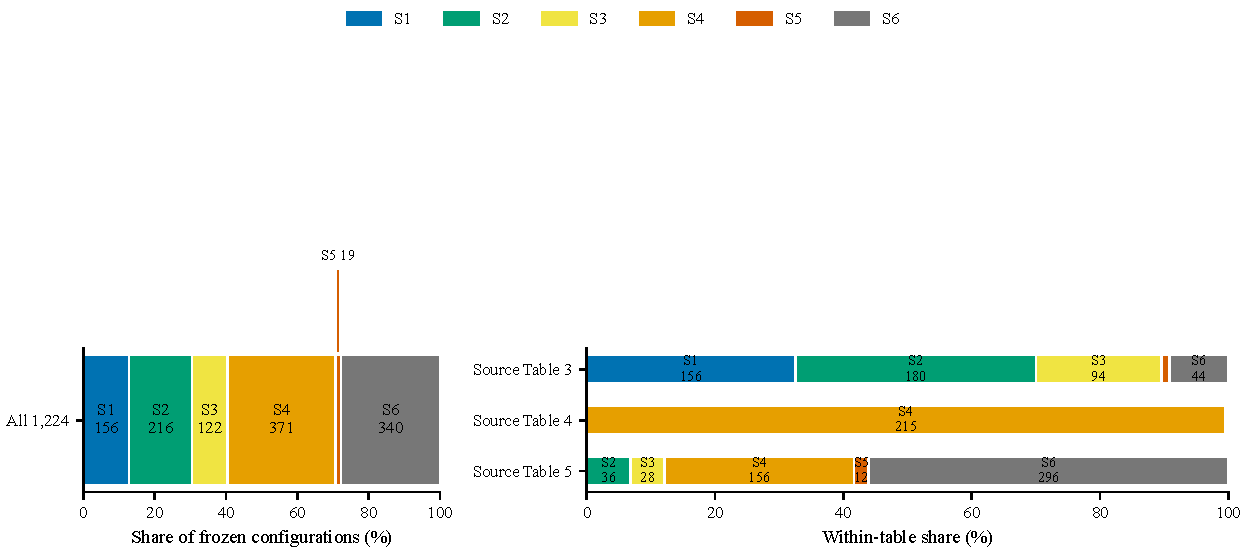
\includegraphics[width=\linewidth]{figures/fig02_configuration_status.pdf}
    \caption{Evidence status in the frozen UrbanEV inventory, overall and by source table.  Completed execution and exact reproduction are separate quantities; status counts do not measure intrinsic model quality.}
    \label{fig:configuration-status}
\end{figure}

\subsection{Fixed fusion recovered part of the oracle gain}
\label{sec:results-accuracy}

The baseline experiment completed all 72 registered runs (three models, six folds, and four horizons).  Among the evaluated single models, compact TimeXer had the lowest macro RMSE at 0.073709.  DLinear reached 0.075362, NLinear 0.075711, and GBDT-Forecaster 0.078165; CAPER's existing same-target result was 0.075507.  TimeXer was best only among the models tested under this UrbanEV protocol.

\begin{table*}[t]
\centering
\caption{Same-protocol UrbanEV accuracy results over six rolling folds and four horizons (24 equal-weight cells, seed 42). The oracle uses target-dependent expert choice and is not deployable.}
\label{tab:accuracy}
\small
\begin{tabular}{lrrrl}
\toprule
Method & Cells & Macro RMSE & Macro MAE & Evidence role \\
\midrule
GBDT-Forecaster & 24 & 0.078165 & 0.049388 & lightweight baseline \\
NLinear & 24 & 0.075711 & 0.047894 & lightweight baseline \\
CAPER & 24 & 0.075507 & 0.048480 & expert \\
DLinear & 24 & 0.075362 & 0.048041 & lightweight baseline \\
TimeXer & 24 & 0.073709 & 0.046367 & best evaluated single model \\
Global Fixed & 24 & 0.071367 & 0.044949 & strict prequential fixed fusion \\
Horizon Fixed & 24 & 0.071372 & 0.044951 & horizon-specific fixed control \\
Oracle & 24 & 0.061233 & 0.035023 & target-dependent upper-bound diagnostic \\
\bottomrule
\end{tabular}
\end{table*}


CAPER and TimeXer still made different local errors, leaving a sizeable oracle gap.  Their mean residual Pearson and Spearman correlations were 0.8422 and 0.7638, respectively.  A target-dependent oracle reduced macro RMSE to 0.061233, a 16.926\% improvement over TimeXer.  This was only an upper bound because it used the realized target to choose the expert.

Global Fixed recovered part of this oracle improvement.  Its macro RMSE was 0.071367, 3.178\% below TimeXer.  It improved all six fold means and all 24 fold--horizon cells, with horizon-level gains from 2.890\% to 3.645\%.  A paired block interval was not part of this earlier frozen accuracy protocol, so the result was not treated as passing the later router or teacher gate.  The Horizon Fixed control was nearly identical at 0.071372.  Post-hoc horizon-specific weights were therefore not needed for the fixed-fusion point result.

Predicting which expert would win was harder than the oracle gap suggested.  A rolling classifier using expert outputs and disagreement alone had mean AUC 0.5370 (range 0.5227--0.5701).  Adding 21 forecast-origin features increased LightGBM mean AUC to 0.6151.  The minimum and maximum fold AUC were 0.5660 and 0.6682, and the mean Brier score was 0.2388.  These proxy results supported running one small router experiment.  They were not evidence of better forecasts.

\subsection{The learned router produced a positive but sub-threshold gain}
\label{sec:results-router}

The hard router underperformed Global Fixed, with macro RMSE 0.072759.  Raw-probability soft routing obtained the lowest observed router RMSE, 0.070979, corresponding to a 0.543\% gain over Global Fixed.  The locked primary direct-loss MLP obtained RMSE 0.071050, a 0.443\% gain.  The better secondary point estimate did not replace that primary comparison.  The MLP won five of six folds and 18 of 24 cells, improved every horizon, and had a paired 24-hour-block gain interval of [0.275\%, 0.634\%].  It captured only 3.123\% of the oracle gap.

Although the consistency checks passed, the 0.443\% gain remained below the frozen 1\% threshold.  Gate 4 therefore failed, and router development stopped.  The result does not show that routing had no signal.  It shows that the measured gain was too small to continue under the registered rule.

\subsection{Global Fixed improved RMSE but increased latency}
\label{sec:results-latency}

The synchronous benchmark completed 90 of 90 process jobs and retained 90,000 raw timing rows.  At batch one, TimeXer required 14.067~ms median and 15.952~ms P95 end-to-end latency.  Global Fixed required 20.940~ms median and 33.123~ms P95.  Thus, the 3.178\% internal RMSE improvement came with 48.86\% higher P50 latency.  P95 latency was also higher.  NLinear and DLinear were much faster (0.674 and 1.166~ms P50) but had higher RMSE.  In this single-GPU sequential workload, Global Fixed had the lowest RMSE, but its latency was substantially higher.  Batch 8/32, model-only, throughput, environment, and portability details appear in the Supplementary Material.

\begin{table}[t]
\centering
\caption{Batch-1 end-to-end accuracy--latency trade-off on the frozen RTX 4060 Laptop GPU, FP32 single-device sequential workload.}
\label{tab:latency}
\small
\begin{tabular}{lrrrr}
\toprule
Method & RMSE & P50 ms & P95 ms & Origins/s \\
\midrule
NLinear & 0.075711 & 0.674 & 1.056 & 1483.7 \\
DLinear & 0.075362 & 1.166 & 1.763 & 857.9 \\
GBDT-Forecaster & 0.078165 & 6.242 & 7.195 & 160.2 \\
CAPER & 0.075507 & 7.934 & 10.798 & 126.0 \\
TimeXer & 0.073709 & 14.067 & 15.952 & 71.1 \\
Global Fixed CAPER+TimeXer & 0.071367 & 20.940 & 33.123 & 47.8 \\
\bottomrule
\end{tabular}
\end{table}


\begin{figure}[t]
    \centering
    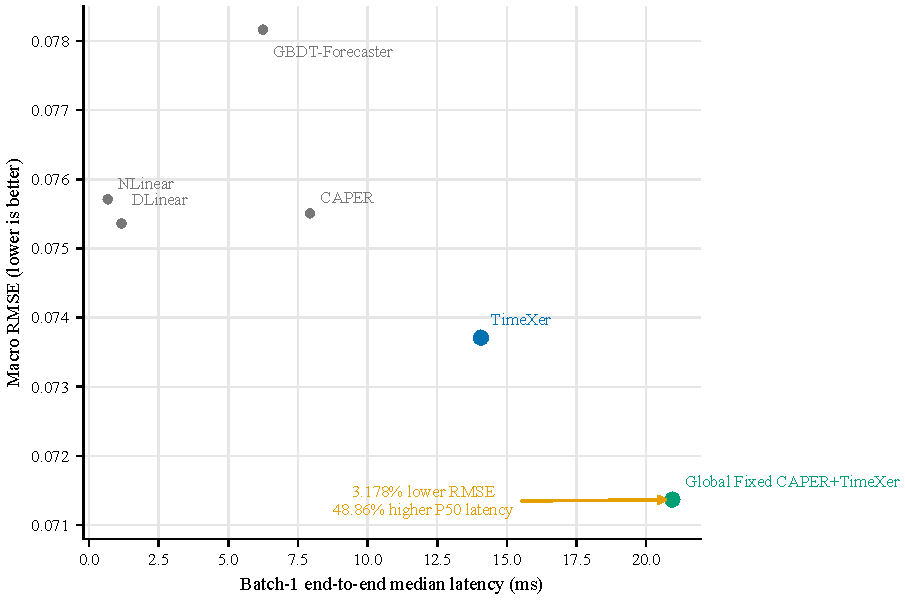
\includegraphics[width=0.82\linewidth]{figures/fig04_accuracy_latency_frontier.pdf}
    \caption{Batch-1 UrbanEV accuracy--latency frontier on the frozen RTX 4060 Laptop GPU in FP32.  The arrow from TimeXer to Global Fixed represents 3.178\% lower RMSE and 48.86\% higher median end-to-end latency.}
    \label{fig:accuracy-latency}
\end{figure}

\subsection{Chronos-2 did not qualify as the UrbanEV teacher}
\label{sec:results-chronos}

The locked Chronos-2 screen completed all 24 fold--horizon cells and 5,960 forecast origins under the zero-shot, no-future-covariate, median point-forecast setting.  Target, index, timestamp, and zone identities passed.  All inputs ended no later than the forecast origin, and a repeated sentinel prediction had maximum absolute difference zero.

Chronos-2 macro RMSE was 0.073542, compared with 0.071367 for Global Fixed, a relative gain of $-3.048\%$.  It beat the control in one of six folds and four of 24 cells.  Its RMSE deteriorated by 2.138\%--3.932\% across the four horizons.  Chronos-2 had lower secondary MAE (0.042250 versus 0.044949), but the registered decision rule used RMSE as the primary endpoint and MAE only as a secondary diagnostic.  Chronos-2 therefore failed this teacher screen, and Global Fixed remained the teacher for this project.  This result is not a general comparison between foundation forecasters and local models.

\subsection{Aligned distillation did not improve consistently over GT-only}
\label{sec:results-distillation}

The final distillation matrix contained 72 audited cells: GT-only, aligned-KD, and shuffled-teacher branches across six folds and four horizons.  Macro RMSE was 0.075568 for GT-only, 0.075478 for aligned KD, and 0.075674 for the shuffled control.  Relative to GT-only, aligned KD improved RMSE by 0.119\%, won four of six folds and 14 of 24 cells, and had a paired interval of [$-0.064\%$, 0.303\%].  It failed the frozen gain, fold, cell, and positive-lower-bound criteria, while horizon protection passed.

Aligned KD did outperform shuffled-teacher training by 0.259\%, with five of six fold wins and a paired interval of [0.151\%, 0.367\%].  This result is consistent with some sample-aligned teacher information, but it did not produce a stable improvement over the identical GT-only student.  The D1 gate failed, \texttt{distill\_v1} terminated, and neither student latency nor multi-seed or protected evaluation was run.

\subsection{Paris gains were consistent but remained below the 1\% rule}
\label{sec:results-paris}

Paris non-available-port-fraction results are reported only within the development boundary and are not compared numerically with UrbanEV.  They are not energy-demand or session-volume forecasts.  Among simple development baselines, last observation had macro RMSE 0.302630, daily lag 0.331654, and weekly lag 0.381137.  Across the 16 fold--horizon cells, the locally audited Paris CAPER adaptation obtained RMSE 0.244601 and the locally audited TimeXer adaptation 0.242542.  The strict prequential fixed teacher reduced RMSE to 0.240488; the target-dependent oracle diagnostic was 0.217661.

The teacher improved over TimeXer by 0.8469\%, won all four folds and all 16 cells, and had a paired interval of [0.6867\%, 1.0088\%].  Every bootstrap replicate selected TimeXer as the best single reference, and no horizon deteriorated.  The result was consistent, but the point estimate remained below the frozen 1\% progression rule.  Because every condition was required, the teacher gate failed.  Student training stopped, the value was not rounded into a pass, and no formal or protected access was authorized.

Formal- and protected-role target-bearing sources existed only in the procedurally isolated evidence vault.  The storage boundary was materialized and hash-audited, but analytical access count remained zero; no post-lock target value or metric from either role contributed to the Paris result or this paper.

\begin{table*}[t]
\centering
\caption{Stage-specific qualification outcomes. Gains use different frozen references and are not absolute cross-stage or cross-dataset comparisons. ``--'' for Chronos-2 means that its frozen screen did not register a paired interval, not zero uncertainty.}
\label{tab:gates}
\scriptsize
\begin{tabular}{llllll}
\toprule
Stage & Frozen reference & Gain & Paired 95\% CI & Primary point gate & Decision \\
\midrule
Router MLP & Global Fixed & +0.443\% & [0.275, 0.634]\% & 1.0\% & FAIL \\
Chronos-2 & Global Fixed & -3.048\% & -- & 1.0\% & FAIL \\
Aligned KD & GT-only student & +0.119\% & [-0.064, 0.303]\% & 1.0\% & FAIL \\
KD vs shuffled & shuffled teacher & +0.259\% & [0.151, 0.367]\% & positive control contrast & PASS SUBCHECK \\
Paris teacher & Paris TimeXer & +0.847\% & [0.687, 1.009]\% & 1.0\% & FAIL \\
\bottomrule
\end{tabular}
\end{table*}


\begin{figure}[t]
    \centering
    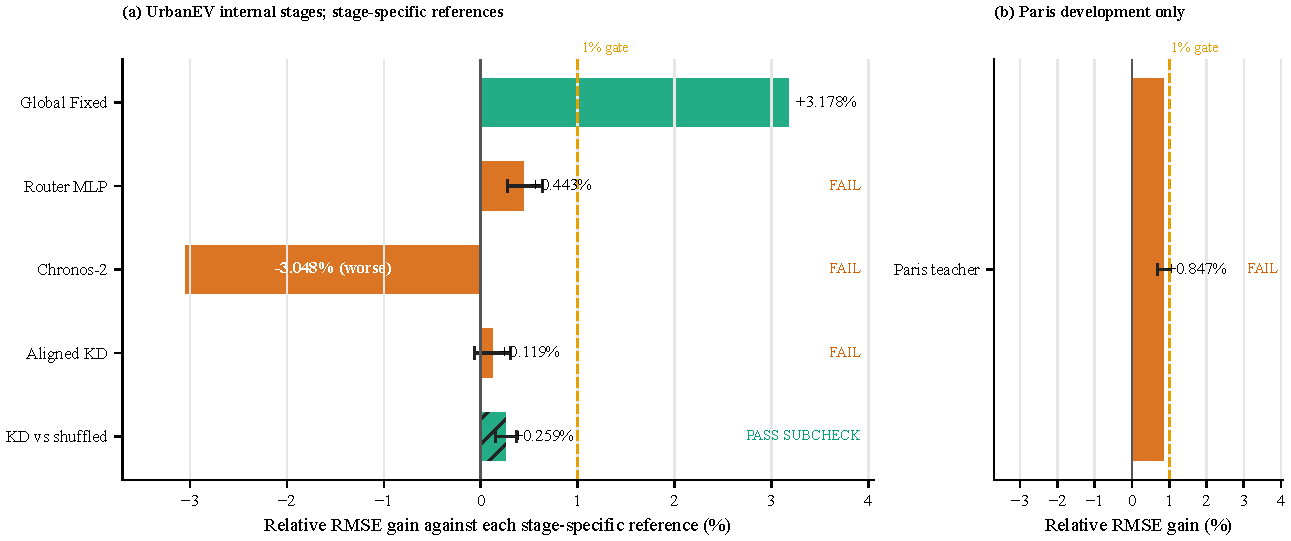
\includegraphics[width=\linewidth]{figures/fig03_stage_gain_gates.pdf}
    \caption{Stage-specific relative gains against each frozen reference.  UrbanEV and Paris use different panels, targets, and references; the plot compares gate outcomes rather than absolute RMSE.  The dashed 1\% line is the project-specific minimum effect, not a universal utility threshold.}
    \label{fig:stage-gains}
\end{figure}

\subsection{Artifact checks blocked metric access until errors were corrected}
\label{sec:results-audit-events}

The first M7-C matrix audit passed 69 of 72 cells and found that three shuffled-control mappings left the data unchanged.  Metrics remained locked.  The pipeline invalidated and reran all 24 shuffled controls instead of rerunning only the three detected cells.  The final audit passed all 72 cells before D1 metrics were computed.

\begin{table*}[t]
\centering
\caption{Fail-closed interventions performed before scientific interpretation. Repairs did not change model predictions or optimize observed metrics.}
\label{tab:audit}
\small
\begin{tabular}{>{\raggedright\arraybackslash}p{0.14\linewidth}>{\raggedright\arraybackslash}p{0.23\linewidth}>{\raggedright\arraybackslash}p{0.27\linewidth}>{\raggedright\arraybackslash}p{0.24\linewidth}}
\toprule
Event & Detection & Required action & Final state \\
\midrule
M7-C control & 3 identity mappings detected (69/72 initial audit pass) & all 24 shuffled controls rerun & 72/72 final audit PASS \\
Paris predeployment review & automated artifact audit: BLOCK & 8 blockers repaired; DEPLOY PASS & pre-run authorization only; metrics locked \\
Paris target repair & 24 runs; 10,236 masked targets restored & restore missing representation; predictions unchanged & metrics still locked \\
Paris metric unlock & 32/32 jobs closed & prediction identity audit & prediction audit PASS; metrics unlocked; teacher gate FAIL; formal/protected analysis locked; analytical access 0 \\
\bottomrule
\end{tabular}
\end{table*}


The Paris pipeline used the same fail-closed rule.  The first automated artifact audit blocked the 32 development runs because eight implementation or boundary requirements were unresolved.  After those issues were corrected, a final automated differential audit issued the internal status \texttt{DEPLOY\_PASS}.  This status authorized the development runs only; it did not indicate deployment readiness.  All 32 model jobs then closed before metric access.

A representation audit later found fill values at masked target positions in 24 of 32 artifacts, covering 10,236 entries.  The repair restored missing-value representation without retraining and left every prediction unchanged.  Metrics had still not been accessed.  A subsequent prediction audit passed 32 of 32 artifacts and then unlocked the development metrics.  These automated audits were not external human replications.

The reported negative decisions were computed only after the registered artifact checks passed.  These checks do not show that auditing improved forecast accuracy.  Throughout the Paris stage, formal and protected sources remained in vault-only storage and the analytical-access count stayed at zero.

\begin{figure}[t]
    \centering
    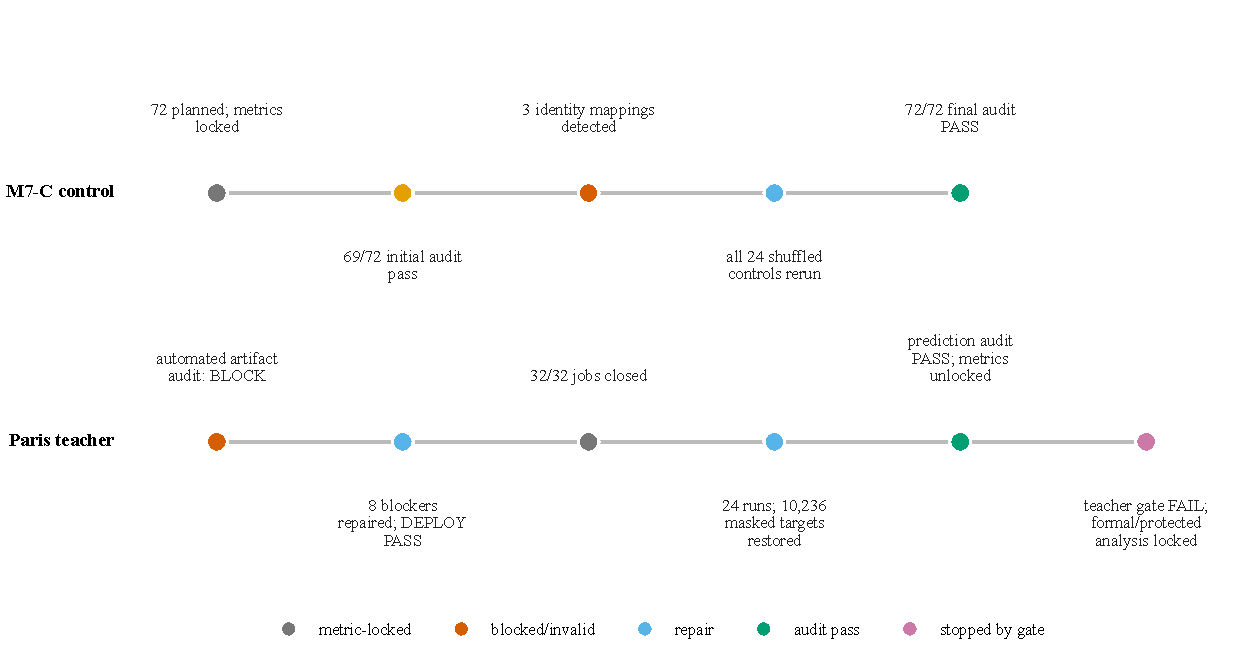
\includegraphics[width=\linewidth]{figures/fig05_audit_timeline.pdf}
    \caption{Fail-closed audit timelines.  Invalid controls and missing-target representation were corrected before metric interpretation; the corrections did not alter model predictions or authorize formal/protected analysis.}
    \label{fig:audit-timeline}
\end{figure}

The Supplementary Material links each research question to its result and supporting artifact.

\section{Discussion}
\label{sec:discussion}

\subsection{Completion does not equal reproduction}

The configuration audit shows a difference that a completed-run count would miss.  Of the 1,224 registered UrbanEV configurations, 865 have completed artifacts, but only 156 meet S1.  S1 requires an identifiable protocol and numerical agreement within the prespecified tolerance.  Other completed artifacts fall into different categories.  Some broadly match the disclosure (S2), some recover only relative trends (S3), and some cannot be mapped to one source configuration (S4).  A successful process exit shows that an implementation ran.  It does not show that the implementation matches the reported experiment.

The status categories also should not be read as model-quality scores.  For example, many S4 entries occur in one source table because identifying information is missing.  That concentration does not show that the associated models are weak.

Using six categories retains more information than a binary ``reproduced/not reproduced'' label.  It keeps partial results separate from exact reproduction and follows prior work that distinguishes artifacts, procedures, and numerical outcomes \cite{pineau2021reproducibility,bouthillier2021variance}.  In this inventory, the difference is visible in the reported rates: 70.67\% of configurations have completed artifacts, whereas 12.75\% meet S1.  These percentages answer different questions.

\subsection{The oracle gap was much larger than the feasible router gain}

CAPER and TimeXer made different local errors.  A target-dependent oracle that selected the lower-error expert for each target reduced RMSE by 16.926\% relative to the best evaluated single model.  The oracle is useful as an upper bound, but it observes the target and cannot be used at forecast time.  When selection was restricted to information available by the forecast origin, the improvement was much smaller.  Global Fixed retained a 3.178\% internal RMSE improvement, while the learned direct-loss router added only 0.443\% over Global Fixed and captured 3.123\% of the oracle gap.

The two values use different information sets.  The first number uses errors observed after the outcome, whereas the second uses only information available before the outcome.  The state-feature classifier's mean AUC of 0.6151 shows moderate ability to predict which expert will have lower error.  It does not show causal knowledge of charging demand or an equivalent forecast gain.  For this reason, we report the oracle, proxy classification, forecast results, and engineering measurements as separate analyses.

The latency measurements add another constraint.  On the frozen RTX 4060 Laptop GPU, batch-one end-to-end P50 latency increased from 14.067 ms for TimeXer to 20.940 ms for Global Fixed, a 48.86\% overhead.  P95 increased from 15.952 to 33.123 ms.  Thus, the result supports an internal accuracy gain with a measured cost on this hardware setup.  It does not support a general deployment recommendation.

\subsection{A positive confidence interval does not satisfy the 1\% rule}

Several experiments produced positive signals but did not meet their predefined rules.  The router improved on Global Fixed by 0.443\%, with a paired 24-hour-block interval of $[0.275\%,0.634\%]$.  The interval is above zero but below the frozen 1\% threshold.  The Paris teacher won all four development folds and all 16 fold--horizon cells.  Its interval was $[0.687\%,1.009\%]$, but its point improvement was 0.847\%.  The rule required a point improvement of at least 1\%, so the teacher did not qualify.  The aligned distillation branch was weaker: its 0.119\% improvement over the identical GT-only student had an interval of $[-0.064\%,0.303\%]$ and failed the fold and cell requirements.

These decisions do not mean that effects below 1\% are scientifically meaningless.  The threshold is a local rule for continuing engineering work, not an operator utility model or a universal statistical constant.  The interval describes uncertainty in the signed effect under the registered bootstrap procedure.  The progression rule asks whether the effect is large and consistent enough to justify another stage.  Using the interval in place of the threshold would change the decision rule after seeing the result.

For context only, a 0.5\% rule would still reject the router, Chronos-2, and aligned KD, but would change the Paris development decision.  A 2\% rule would reject every downstream candidate.  These calculations do not change the frozen 1\% decisions.

\subsection{Stopping rules limited repeated search on the same data}

The stopping rules prevented small positive results from starting open-ended searches on the same evidence interval.  Router v1 stopped after its effect-size failure.  Chronos-2 remained a recorded zero-shot teacher screen after its $-3.048\%$ gain against Global Fixed.  Distillation v1 stopped after the aligned branch failed its main rule, even though it beat the shuffled control by 0.259\%.  The Paris teacher also stopped at development; formal and protected targets were not opened after the near-threshold result.  Each negative result therefore corresponds to a prespecified comparison rather than one step in an unreported adaptive search \cite{cawley2010selectionbias,dwork2015reusableholdout}.

The artifact checks had a similar role.  In the distillation matrix, three identity mappings invalidated the shuffled controls while metrics remained locked.  All 24 shuffled-control cells were rerun, and metrics were unlocked only after the 72/72 audit passed.  In Paris, the first automated predeployment audit blocked execution on eight issues.  After correction, 32 prediction artifacts closed without evaluation metrics.  A later representation audit changed 10,236 masked target entries back to missing values across 24 runs without changing predictions.  Metrics remained locked until all 32 artifacts passed the identity audit.  These repairs ensure that the reported metrics use the intended artifacts.  They do not show that repair improved model accuracy.

\subsection{The vault records data separation, not model performance}

Paris formal and protected target-bearing files are stored outside the main project.  The inventory contains 48 non-self-referential files, including 29 hidden Git files and the object pack that could reconstruct removed target sources.  Every entry matches its recorded byte count and SHA-256 hash.  The formal and protected shards cover 2020-12-01 through 2021-01-19 and 2021-01-20 through 2021-03-10.  The files were moved once, but the protected analytical-access count remains zero.  Failed partial files are also inventoried and were not analyzed.

This record supports one limited claim: no post-lock Paris formal or protected target contributed to model selection, metric computation, or a paper result.  It does not mean that the bytes never existed, that two pre-lock schema rows were never visible, or that Paris development is a blind test.  The controls address accidental analysis, stale-cache reuse, path leakage, and recoverable Git history.  They do not protect against a malicious authenticated user or an operating-system compromise, and the vault is not encrypted storage.  Its purpose is to make the zero-access statement checkable and to retain the targets for a later versioned protocol.

\subsection{Practical reporting suggestions}

Based on this case, authors should state whether a target measures energy, sessions, active charging, occupancy, or port non-availability.  They should also report denominators and observation masks, keep model-search periods separate from later operational evaluation, and define the request shape used for latency.  Reviewers can then check whether a completed run is still underidentified, whether an oracle or proxy is being reported as forecast performance, and whether a positive interval is being used in place of a predefined minimum-effect rule.

Operational studies may also need measures beyond macro RMSE, such as peak-period error, high-occupancy recall, calibrated intervals, or denied-service proxies.  This paper does not estimate those quantities.  The Supplementary Material contains an author/reviewer checklist derived from this case.

\section{Limitations}
\label{sec:limitations}

\paragraph{Scope of the registry.}
The 1,224-configuration taxonomy describes one frozen UrbanEV reproduction inventory. Its S1--S6 assignments depend on the available source disclosure, deterministic mapping rules, and internally fixed 2\% and 5\% numerical tolerances. The classifications were not independently double-coded, and no inter-rater reliability estimate is available. The resulting 12.75\% S1 rate is not an estimate of reproducibility across urban forecasting as a field. Status counts also measure evidence identifiability and execution state, not intrinsic model quality.

\paragraph{Framework validation.}
The proposed audit framework is extracted from a single self-audited project. Separately instantiated automated artifact audits challenged specific protocol and result packages, but they were not external human replications, and no external team has applied the full claim grammar, state machine, or S1--S6 decision tree to a separate benchmark. The paper therefore offers a reusable instrument and worked case, not evidence that the instrument improves decisions or reduces false discoveries across laboratories.

\paragraph{Internal and development-only evaluation.}
The UrbanEV comparisons use six internal rolling folds, four horizons, and seed 42. Paris teacher qualification uses four development folds over a different panel, non-available-port target, missingness mask, and local audited model adaptations. Absolute UrbanEV and Paris RMSE values are therefore not comparable. The windows also differ behaviorally: Shenzhen covers September 2022--February 2023, whereas Paris development covers July--November 2020, when pandemic-era mobility, policy, infrastructure, pricing, land use, and fleet composition could differ. The evidence controls protocol leakage, not those transport-domain shifts. No UrbanEV protected evaluation was opened, and no post-lock Paris formal or protected target was used analytically. The results do not establish blind-test generalization, robustness across seeds or cities, production readiness, or state of the art.

\paragraph{Restricted candidate and implementation set.}
The baseline conclusion applies only to the evaluated candidates. The Chronos-2 screen fixes one official model revision, zero-shot FP32 inference, and no future covariates; it does not establish that foundation models generally underperform on charging data. Likewise, the CAPER and compact TimeXer Paris implementations are local audited adaptations rather than claims about every upstream implementation. The residual-distillation result concerns one 338-parameter student and one seed, and the stopped protocol did not authorize a student architecture search, multi-seed expansion, or latency evaluation.

\paragraph{Oracle, proxies, and uncertainty.}
The oracle is target-dependent and only bounds latent complementarity. The expert-advantage classification task uses a proxy label derived from relative expert errors; its AUC does not prove causal predictability or forecast improvement. Paired block-bootstrap intervals account for temporal dependence under the chosen 24-hour blocking scheme, but they do not eliminate all uncertainty from fold construction, model selection, or a small number of seeds. Each Paris fold retained a trailing 12-hour partial block, and no post-hoc 48- or 168-hour sensitivity was run, so its interval should be interpreted under that exact resampling implementation. The 1\% minimum-effect gate is a project-specific progression rule without an accompanying economic utility model, and it should not be generalized as a universal significance threshold.

\paragraph{Hardware-specific latency.}
Latency was measured in FP32 under single-device sequential execution on one RTX 4060 Laptop GPU; batch one was the frozen primary endpoint, while batches 8 and 32 are descriptive appendices. A request produced predictions for 275 zones and four horizons. Kernel fusion, parallel expert execution, quantization, compilation, batching, cold start, a different accelerator, or a serving system could change both the absolute timings and the fusion overhead. The measured 48.86\% P50 overhead is reproducible for the frozen warm-resident workload, not portable to arbitrary deployments.

\paragraph{Audit coverage.}
Fail-closed checks detected identity shuffles, target-representation errors, incomplete provenance, and premature metric access. These checks reduce known integrity risks but cannot prove the absence of every implementation defect. The repairs were verified through hashes, identities, and unchanged predictions; they were not independently reimplemented from scratch. The automated Paris result artifact audit retained non-decisive warnings: the teacher-weight CSV did not carry complete upstream provenance, the pre-unlock state lacked a separate hash snapshot, and the receipt-update chain was weaker than the prediction-identity audit itself. None can reverse a point estimate below the frozen gate, but they limit stronger process claims. Two example source rows were displayed during early schema discovery before the Paris boundary lock, when no model or selection rule existed. This event was logged and was not used for model choice, but it prevents an absolute claim that no target value was ever visible before boundary creation.

\paragraph{Dataset-license metadata.}
The Paris challenge repository and the associated Zenodo record expose different license labels (ODbL and CC BY 4.0, respectively) \cite{amaraouali2024smarter,amaraouali2023parisdataset}. This paper treats them as source-specific metadata and does not resolve the legal relationship between the records. Downstream redistribution should therefore verify the applicable terms at the exact source used.

\paragraph{Vault boundary.}
The final vault manifest covers 48 non-self-referential files, including 29 Git files, and all recorded hashes verify. Analytical access to protected labels is zero, but storage migration materialized formal and protected shards and retained redundant raw, reference, final-shard, and failed-partial copies. The partials were inventoried but not analyzed. The vault inherits filesystem permissions, including modify rights for authenticated users; it is procedural isolation rather than encryption or hardened authorization. Some truth-derived tutorial figures and score summaries remain outside the exact-target isolation set because they cannot reconstruct station-level labels. These properties limit the claim to verified source separation and zero analytical use.

\paragraph{Negative-result interpretation.}
A failed frozen gate does not prove that an entire method family cannot work. It establishes only that the audited candidate, reference, data interval, and qualification rule did not authorize progression. Conversely, a passed subcheck---such as aligned distillation outperforming a shuffled teacher---does not upgrade the failed main comparison. Our conclusions concern the evidential status of these experiments, not universal impossibility.

\section{Conclusion}
\label{sec:conclusion}

This study considered four questions separately: whether a configuration is identifiable, whether an implementation completed, whether it carries predictive signal, and whether its gain meets the rule for moving to the next stage.  In the UrbanEV registry, 865 of 1,224 configurations have completed artifacts, but only 156 meet S1.  Completion is useful information, but it is not the same as exact reproduction.

The later model experiments produced different results at each stage.  The target-dependent oracle reduced RMSE by 16.926\% relative to TimeXer.  Strict prequential fixed fusion retained a 3.178\% internal gain and increased batch-one P50 latency by 48.86\% on the frozen device.  Learned routing, the Chronos-2 teacher screen, aligned residual distillation, and the Paris development teacher were each evaluated under their registered rules, but none met its progression rule.  Positive router and Paris intervals did not replace the project-specific 1\% point requirement.

Metric locks, full control reruns, prediction-identity checks, and time-stamped stopping rules made each negative result traceable to a prespecified comparison.  Paris formal and protected targets were kept out of the present analysis.  The separate store contains 48 non-self-referential files, including 29 recoverable Git files, and the protected analytical-access count remains zero.  This is a documented storage rule; it is not encrypted storage or a protected-test result.

The main result concerns evaluation practice rather than a new model architecture.  In this case, separate checks make clear which conclusions the stored evidence supports.  The wording rules and audit checklist have not yet been tested by another team or on another benchmark.  Future work should apply a newly frozen model and loss specification to an untouched data boundary, use multiple seeds and hardware environments, and test the same stopping rules independently.  At present, the evidence supports an internal accuracy--cost result and the recorded negative decisions, while formal and protected targets remain unused for later evaluation.  It does not support a state-of-the-art or deployment-readiness claim.

\section*{Data and artifact availability}
The public repository contains versioned source snapshots, protocol/configuration locks, target-free prediction artifacts, machine-readable result summaries, and scripts that reconstruct the headline metrics after the user obtains the licensed source datasets. Paris formal and protected targets, raw reference files, recoverable Git objects, and private vault metadata are not distributed. Their public boundary receipt contains only role dates, hashes, row counts, and the zero analytical-access statement.
\section*{Funding}
This research received no external funding.
\section*{Competing interests}
The author declares no competing interests.
\section*{Ethics and scope statement}
The study uses previously released charging datasets and contains no intervention on human participants. Charging observations may nevertheless encode mobility patterns, so the paper reports only aggregate forecasting evidence and does not attempt individual inference. No protected-test, deployment-readiness, or state-of-the-art claim is made.
\section*{AI assistance disclosure}
Generative AI tools, including OpenAI Codex and ChatGPT, assisted with literature search, experiment-script development, artifact-consistency checks, separately instantiated automated artifact audits, figure preparation, and language editing. All reported numerical results were computed from stored predictions and licensed source targets by deterministic scripts. AI tools did not generate ground-truth targets, alter frozen thresholds, authorize formal or protected data access, or determine the final scientific claims. The confirmed first author reviewed the manuscript and accepts responsibility for its content.
\begingroup
\sloppy
\small
\setlength{\emergencystretch}{10em}
\bibliographystyle{unsrtnat}
\bibliography{../shared/references}
\endgroup
\end{document}
